% Source: Complex.pdf, pages 1-8. Title on the source: "Statistical mechanics with complexified
% physical parameters". The notes carry no lecture number.
\subsection{Complex parameters and Lee--Yang zeros}
\subsubsection*{Complex variables and series expansions}

In mathematics, it is often useful to generalize from functions of a real variable to functions of a
complex variable, $\mathbb R\to\mathbb C$. For example, in general, one must make this step when solving for
the roots of an algebraic equation with real coefficients. Consider the quadratic equation
$ax^2+bx+c = 0$. The solutions are $x = (1/(2a))\left[-b\pm\sqrt{b^2-4ac}\right]$ and these are complex if
$b^2<4ac$. This generalization is also necessary to understand the properties of series expansions. For
instance, consider the Taylor series expansion
\begin{equation}
  f(x) = \frac{1}{1+x^2} = \sum_{n=0}^\infty(-x^2)^n\qquad\text{with } x\in\mathbb R .
\end{equation}
Although $f(x)$ is well-behaved $\forall\,x\in\mathbb R$, the series diverges if $x<-1$ or $x>1$. This seems
puzzling if one restricts attention to real $x$, since $f(x)$ is well behaved and actually gets smaller as $|x|$
increases through 1. An understanding of this requires that one generalize $x$ from $x\in\mathbb R$ to
$x\in\mathbb C$; then one sees that $f(x)$ has poles at $x = \pm\ii$. These poles set the radius of convergence of
the Taylor series for $f(x)$.

\begin{diagram}
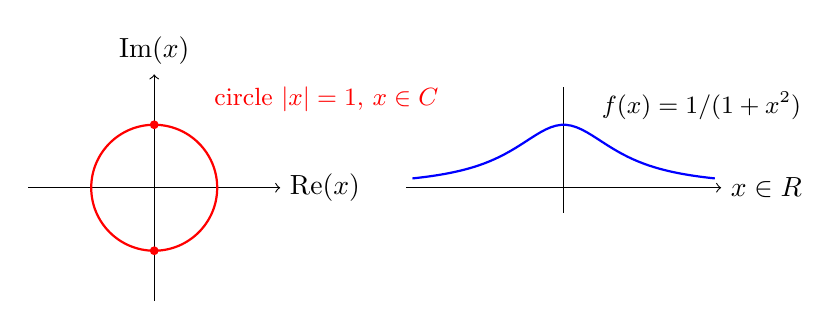
\begin{tikzpicture}[scale=0.8]
  \draw[->] (-2,0) -- (2,0) node[right] {$\mathrm{Re}(x)$}; \draw[->] (0,-1.8) -- (0,1.8) node[above] {$\mathrm{Im}(x)$};
  \draw[red,thick] (0,0) circle (1); \fill[red] (0,1) circle (0.07); \fill[red] (0,-1) circle (0.07);
  \node[red,font=\small,anchor=west] at (0.8,1.4) {circle $|x| = 1$, $x\in\mathbb C$};
  \begin{scope}[xshift=6.5cm]
  \draw[->] (-2.5,0) -- (2.5,0) node[right] {$x\in\mathbb R$}; \draw (0,-0.4) -- (0,1.6);
  \draw[thick,blue,domain=-2.4:2.4,samples=60] plot (\x,{1.0/(1+\x*\x)});
  \node[font=\small,anchor=west] at (0.45,1.3) {$f(x) = 1/(1+x^2)$};
  \end{scope}
\end{tikzpicture}
\diagramcaption{The poles of $f(x) = 1/(1+x^2)$ at $x = \pm\ii$ lie on the circle $|x| = 1$ in the complex plane
(left), although $f$ is smooth on the real axis (right).}
\end{diagram}

\subsubsection*{Lee--Yang zeros in the complex field plane}

One also gains insight by studying statistical mechanical models with the physical parameters generalized from
$\mathbb R$ to $\mathbb C$. T.D.~Lee and C.N.~Yang pioneered the generalization of the external magnetic field to
complex values (1952) and M.E.~Fisher considered the generalization of $K = \beta J$ to complex values (1965). Let
us consider the Ising model first, with $\Ham = -J\sum_{nn}\sigma_i\sigma_j - H\sum_i\sigma_i$, with $J>0$, on a
lattice $\Lambda$. Then
\begin{equation}
  Z = \sum_{\{\sigma_i\}}e^{-\beta\Ham} = \sum_{\{\sigma_i\}}e^{K\sum_{nn}\sigma_i\sigma_j + h\sum_i\sigma_i},
  \qquad K = \beta J,\quad h = \beta H .
\end{equation}
At $T = 0$, $Z = 2e^{(\Delta/2)Kn+hn}$, where $\Delta$ = vertex degree of $\Lambda$. Recall the low-temperature
expansion:
\begin{equation}
  Z = e^{n\left((\Delta/2)K+h\right)}\left[1 + nz^\Delta\mu + \cdots\right],\qquad\text{where}\quad z = e^{-2K}\ \text{and}\ \mu = e^{-2h}.
\end{equation}
It is thus clear that aside from the prefactor, $Z$ is a polynomial in the Boltzmann weights $z = e^{-2K}$ and
$\mu = e^{-2h}$. By multiplying by a different prefactor, one could also write $Z$ as a polynomial in
$z^{-1} = e^{2K}$ and $\mu^{-1} = e^{2h}$.

An interesting question concerns the zeros of the partition function $Z$ in $z$ for fixed $\mu$ and the zeros in
$\mu$ for fixed $z$. Lee and Yang showed that for the ferromagnetic case, the zeros of $Z$ in $\mu$ for fixed
(physical) $z$, i.e.\ $0\le z\le 1$ (i.e.\ $T = 0$, $K = \infty\Rightarrow z = 0$ and $T = \infty$,
$K = 0\Rightarrow z = 1$), lie on the unit circle in the complex $\mu$ plane (Phys.\ Rev.\ \textbf{87}, 404, 410
(1952)). At $T = \infty$, these zeros are all clustered at $\mu = -1$. As $T$ decreases from $\infty$, they move
out along the unit circle. The locus of zeros is invariant under complex conjugation since the coefficients of
terms in $Z$ are real. In the thermodynamic limit, these zeros are dense on the complex-conjugate arcs of the
unit circle. If $\Lambda$ has dimension above $d = 1$, i.e.\ $d\ge 2$, so that the model has a critical point at
$T_c>0$, then as $T\searrow T_c$, the complex-conjugate arcs ``pinch'' the real axis at $\mu = 1$, thereby forming
a closed curve (the unit circle) that separates the complex $\mu$ plane into 2 regions, $|\mu|>1$ and $|\mu|<1$.
So $\mu = e^{\ii\theta} = e^{-2h}$; $h = -\ii\theta/2$.

\begin{diagram}
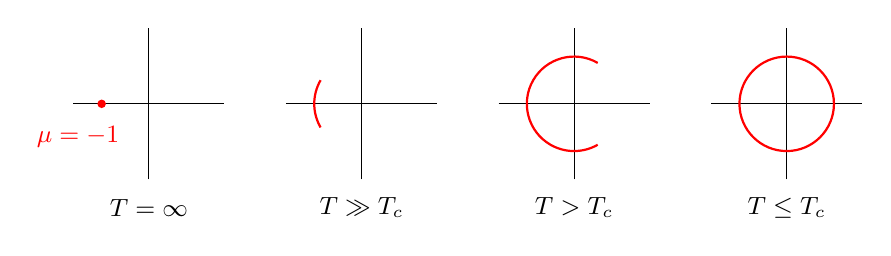
\begin{tikzpicture}[scale=0.6]
  \foreach \s/\lab/\a in {0/{$T = \infty$}/180, 4.5/{$T\gg T_c$}/150, 9/{$T>T_c$}/60, 13.5/{$T\le T_c$}/0} {
    \begin{scope}[xshift=\s cm]
      \draw (-1.6,0) -- (1.6,0); \draw (0,-1.6) -- (0,1.6);
      \ifdim\a pt=180pt \fill[red] (-1,0) circle (0.09);
      \else \draw[red,thick] (\a:1) arc (\a:360-\a:1); \fi
      \node[font=\small] at (0,-2.2) {\lab};
    \end{scope}}
  \node[red,font=\small] at (-1.5,-0.7) {$\mu = -1$};
\end{tikzpicture}
\diagramcaption{Lee--Yang zeros (red) in the complex $\mu$ plane, on $|\mu| = 1$, $\mu\in\mathbb C$, as $T$
decreases.}
\end{diagram}

The zeros thus occur for a range of $\theta$ starting at $\theta = \pm\pi$ extending to $\pi\ge|\theta|>\theta_e$,
where $e$ denotes endpoint.

\paragraph{Example.} Recall the 1D Ising model, with transfer matrix
$T = \left(\begin{smallmatrix}e^{K+h} & e^{-K}\\ e^{-K} & e^{K-h}\end{smallmatrix}\right)$ and eigenvalues
\begin{equation}
  \lambda_\pm = e^K\left[\cosh h\pm\sqrt{\sinh^2h+e^{-4K}}\right].
\end{equation}
Let $h = -\ii\theta/2$ and use the identities $\cosh(\ii x) = \cos x$, $\sinh(\ii x) = \ii\sin x$. Here
$Z = \lambda_+^n+\lambda_-^n$; the zeros require $|\lambda_+| = |\lambda_-|$ for cancellation. For physical $K$, $h$,
$\lambda_+>\lambda_-$, so $Z$ is never zero, as is obvious from the definition $Z = \sum_{\{\sigma\}}e^{-\beta\Ham}$,
which is positive-definite, but $Z$ can vanish for complex $h$ and/or $K$. Setting $h = -\ii\theta/2$,
\begin{equation}
  \lambda_\pm\to e^K\left[\cos\frac{\theta}{2}\pm\sqrt{-\sin^2(\theta/2)+e^{-4K}}\right];
\end{equation}
$|\lambda_+| = |\lambda_-|$ if the expression in the square root is negative, i.e.\
$\sin^2(\theta/2)>e^{-4K}$, $|\sin\theta/2|>e^{-2K}$. For the $\theta>0$ branch of the arc,
$\theta/2>\arcsin(e^{-2K})$, with the endpoints of the arc at
\begin{equation}
  \theta_e = \pm 2\arcsin(e^{-2K}).
\end{equation}
E.g.\ $T = \infty$, i.e.\ $K = 0\Rightarrow e^{-2K} = 1$, $\theta_e = \pm 2\left(\pi/2\right) = \pm\pi$; as $T\to 0$,
$K\to\infty$, $e^{-2K}\to 0$, $\theta_e\to 0$.

\begin{diagram}
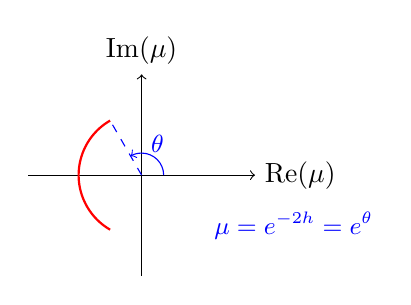
\begin{tikzpicture}[scale=0.8]
  \draw[->] (-1.8,0) -- (1.8,0) node[right] {$\mathrm{Re}(\mu)$}; \draw[->] (0,-1.6) -- (0,1.6) node[above] {$\mathrm{Im}(\mu)$};
  \draw[red,thick] (120:1) arc (120:240:1);
  \draw[blue,dashed] (0,0) -- (120:1); \draw[blue,->] (0.35,0) arc (0:120:0.35); \node[blue,font=\small] at (0.25,0.5) {$\theta$};
  \node[blue,font=\small,anchor=west] at (1.0,-0.8) {$\mu = e^{-2h} = e^{\ii\theta}$};
\end{tikzpicture}
\diagramcaption{The arc of Lee--Yang zeros for the 1D Ising model, with endpoints at $\theta_e = \pm 2\arcsin(e^{-2K})$.}
\end{diagram}

\subsection{Fisher zeros in the complex temperature plane}

Complex-$K$ zeros are also of interest. In general, with $Z = \Tr(T^n) = \sum_i\lambda_i^n$, so
$f = \lim_{n\to\infty}(1/n)\ln Z = \ln(\lambda_{\text{dom.}})$; at the locus of points where there is a switch in
the dominant eigenvalue, where $|\lambda_i| = |\lambda_j|$ for some $i$, $j$, as occurs for zeros of $Z$, there is a
nonanalytic change in the (reduced) free energy $f$. This establishes a connection between the accumulation set of
the zeros of $Z$ and the complex-$K$ generalization of phase transition points $K_c$.

One can relate this to singularities of an integral representation for $f$. Let us illustrate this by focussing on
a switch between 2 dominant eigenvalues of $T$, so let $Z = \lambda_1^n+\lambda_2^n$. Now, assuming $n$ even,
\begin{align}
  \lambda_1^n+\lambda_2^n &= \prod_{\ell=0}^{n-1}\left(\lambda_1 + e^{(2\ell+1)\ii\pi/n}\lambda_2\right)
   = \prod_{\ell=0}^{n/2-1}\left(\lambda_1 + e^{(2\ell+1)\ii\pi/n}\lambda_2\right)\left(\lambda_1 + e^{-(2\ell+1)\ii\pi/n}\lambda_2\right)\nonumber\\
  &= \prod_{\ell=0}^{n/2-1}\left[\lambda_1^2+\lambda_2^2+2\lambda_1\lambda_2\cos\left(\frac{(2\ell+1)\pi}{n}\right)\right],
\end{align}
so, for $n\to\infty$,
\begin{equation}
  f = \lim_{n\to\infty}\frac{1}{n}\ln Z = \frac{1}{2}\int_0^{2\pi}\frac{\dd\theta}{2\pi}\ln\left[\lambda_1^2+\lambda_2^2+2\lambda_1\lambda_2\cos\theta\right]
  = \ln[\lambda_{\text{dom.}}];
\end{equation}
the integrand is singular where $|\lambda_1| = |\lambda_2|$, i.e.\ on the locus of zeros of $Z$ for
$\lambda_i\in\mathbb C$.

\paragraph{1D Ising model.} Recall the 1D Ising model with $H = 0$: $Z = \lambda_+^n+\lambda_-^n$,
$\lambda_\pm = e^K\pm e^{-K}$. The condition for equality of eigenvalues, $|\lambda_+| = |\lambda_-|$, is
$|e^K+e^{-K}| = |e^K-e^{-K}|$, i.e.\ $|1+e^{-2K}| = |1-e^{-2K}|$, i.e.\ $|1+z| = |1-z|$, where $z = e^{-2K}$
(don't confuse it with $Z$). Solution: $z$ pure imaginary, $z = \ii r$, $r\in\mathbb R$. So the locus of zeros of
$Z$ in the thermodynamic limit is the imaginary axis in the complex $z$ plane. This locus separates the complex $z$
plane into 2 regions, $\mathrm{Re}(z)>0$ and $\mathrm{Re}(z)<0$. Denote this locus as $\mathcal B_z$ ($\mathcal B$
stands for ``boundary''). With $J>0$, this locus $\mathcal B_z$ crosses the real $z$ axis at $z = 0$, i.e.\
$K = \infty$, i.e.\ $T = 0$ (and also at $|z| = \infty$, i.e.\ $K = -\infty$, i.e.\ $T = 0$ with $J<0$ (AFM)). So
these crossings occur at the critical point of this 1D model, at $T = 0$ for the respective FM ($J>0$) and AFM
($J<0$) cases. The fact that the coefficients of terms in $Z$ are real $\Rightarrow\mathcal B_z = \mathcal B_z^*$,
i.e.\ the locus $\mathcal B_z$ is invariant under complex conjugation. The isomorphism of the FM and AFM on a
bipartite lattice such as the 1D line (with $n$ even) $\Rightarrow\mathcal B_z$ is also invariant under
$z\to z^{-1}$, inversion, corresponding to $J\to-J$ (so $K\to-K$, $z\to1/z$).

\paragraph{2D Ising model.} The locus of complex-$K$ zeros for the 2D Ising model can be determined from the exact
solution, as the locus in $z$ or $v$ where the argument of the log in the integral vanishes, similarly to the 1D
integral. Recall, for the square lattice,
\begin{equation}
  f = 2K + \frac{1}{2}\int_0^{2\pi}\frac{\dd^2\theta}{(2\pi)^2}\ln(L),\qquad
  L = (1+z^2)^2 - 2z(1-z^2)\mathcal P(\theta_1,\theta_2),
\end{equation}
with $\mathcal P(\theta_1,\theta_2) = \cos\theta_1+\cos\theta_2$; $-2\le\mathcal P(\theta_1,\theta_2)\le 2$. As
$0\le\theta_1,\theta_2\le 2\pi$ and $-2\le\mathcal P\le 2$, the solutions to the equation $L = 0$ sweep out curves in
the complex-$z$ plane. These form 2 circles, $|z\pm1| = \sqrt2$, which cross the real axis at
$z_{PM\text{-}FM} = \sqrt2-1$, $z_{PM\text{-}AFM} = (z_{PM\text{-}FM})^{-1} = \sqrt2+1$, and 2 other points.

\begin{diagram}
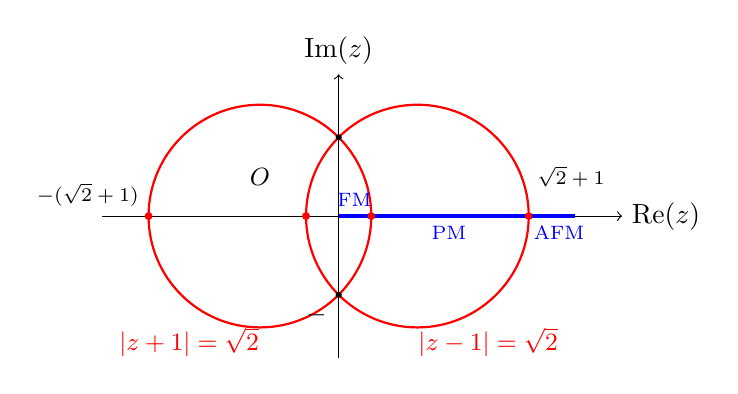
\begin{tikzpicture}[scale=1.0]
  \draw[->] (-3,0) -- (3.6,0) node[right] {$\mathrm{Re}(z)$}; \draw[->] (0,-1.8) -- (0,1.8) node[above] {$\mathrm{Im}(z)$};
  \draw[red,thick] (-1,0) circle (1.414); \draw[red,thick] (1,0) circle (1.414);
  \draw[very thick,blue] (0,0) -- (0.414,0); \draw[very thick,blue] (0.414,0) -- (2.414,0); \draw[very thick,blue] (2.414,0) -- (3,0);
  \fill[red] (0.414,0) circle (0.05); \fill[red] (2.414,0) circle (0.05); \fill[red] (-0.414,0) circle (0.05); \fill[red] (-2.414,0) circle (0.05);
  \node[blue,font=\scriptsize,above] at (0.2,0) {FM}; \node[blue,font=\scriptsize,below] at (1.4,0) {PM}; \node[blue,font=\scriptsize,below] at (2.8,0) {AFM};
  \node[font=\scriptsize,above right] at (2.4,0.25) {$\sqrt2+1$};
  \node[font=\scriptsize,above left] at (-2.414,0) {$-(\sqrt2+1)$};
  \fill (0,1) circle (0.04); \fill (0,-1) circle (0.04);
  \node[font=\small,anchor=south east] at (-0.03,1.03) {$\ii$}; \node[font=\small,anchor=north east] at (-0.03,-1.03) {$-\ii$};
  \node[red,font=\small] at (-1.9,-1.6) {$|z+1| = \sqrt2$}; \node[red,font=\small] at (1.9,-1.6) {$|z-1| = \sqrt2$};
  \node[font=\small] at (-1,0.5) {$O$};
\end{tikzpicture}
\diagramcaption{The boundary $\mathcal B_z$ for the square-lattice Ising model (not exactly to scale), with the
physical phases marked in blue: PM, $\sqrt2-1\le z\le 1$ for $J>0$, $1\le z\le\sqrt2+1$ for $J<0$; FM,
$0\le z<\sqrt2-1$; AFM, $z>\sqrt2+1$.}
\end{diagram}

$\mathcal B_z$ is invariant under (1) $z\to z^*$; (2) $z\to1/z = y$; (3) $z\to-z$. This boundary
$\mathcal B_z$ thus defines complex-$z$ extensions of the physical phases.

Recall that $v = (1-z)/(1+z)$ maps the $z$ plane to the $v$ plane. This mapping takes
$\mathcal B\to\mathcal B$, so $\mathcal B_v$ is the same as $\mathcal B_z$: $|v\pm1| = \sqrt2$, although the
crossings on the real-$z$ and real-$v$ axes correspond to different phase transitions. With $v = \tanh K$, the
physical phases are: $0\le v\le\sqrt2-1$: PM for $J>0$; $-(\sqrt2-1)\le v\le 0$: PM for $J<0$;
$\sqrt2-1<v<1$: FM for $J>0$; $-1<v<-(\sqrt2-1)$: AFM for $J<0$.

\begin{diagram}
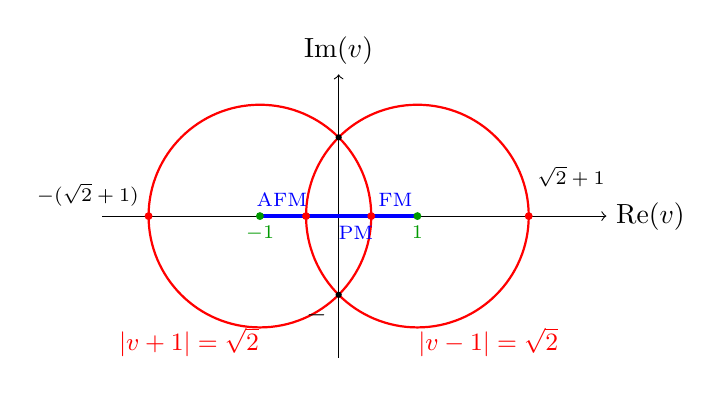
\begin{tikzpicture}[scale=1.0]
  \draw[->] (-3,0) -- (3.4,0) node[right] {$\mathrm{Re}(v)$}; \draw[->] (0,-1.8) -- (0,1.8) node[above] {$\mathrm{Im}(v)$};
  \draw[red,thick] (-1,0) circle (1.414); \draw[red,thick] (1,0) circle (1.414);
  \draw[very thick,blue] (-1,0) -- (1,0);
  \fill[red] (0.414,0) circle (0.05); \fill[red] (2.414,0) circle (0.05); \fill[red] (-0.414,0) circle (0.05); \fill[red] (-2.414,0) circle (0.05);
  \fill[green!60!black] (1,0) circle (0.05); \fill[green!60!black] (-1,0) circle (0.05);
  \node[blue,font=\scriptsize,below] at (0.22,0) {PM}; \node[blue,font=\scriptsize,above] at (0.72,0) {FM}; \node[blue,font=\scriptsize,above] at (-0.72,0) {AFM};
  \node[green!60!black,font=\scriptsize,below] at (1,0) {$1$}; \node[green!60!black,font=\scriptsize,below] at (-1,0) {$-1$};
  \node[font=\scriptsize,above right] at (2.4,0.25) {$\sqrt2+1$};
  \node[font=\scriptsize,above left] at (-2.414,0) {$-(\sqrt2+1)$};
  \fill (0,1) circle (0.04); \fill (0,-1) circle (0.04);
  \node[font=\small,anchor=south east] at (-0.03,1.03) {$\ii$}; \node[font=\small,anchor=north east] at (-0.03,-1.03) {$-\ii$};
  \node[red,font=\small] at (-1.9,-1.6) {$|v+1| = \sqrt2$}; \node[red,font=\small] at (1.9,-1.6) {$|v-1| = \sqrt2$};
\end{tikzpicture}
\diagramcaption{The boundary $\mathcal B_v$, with the physical phases on the real $v$ axis marked in blue: PM for
$|v|\le\sqrt2-1$, FM for $\sqrt2-1<v<1$, AFM for $-1<v<-(\sqrt2-1)$.}
\end{diagram}

Thermodynamic quantities can be formally analytically continued from physical $z$ or $v$ values to complex-$K$ values.
For example, the spontaneous magnetization of the 2D Ising model on the square lattice:
\begin{equation}
  M = (1-k_<^2)^{1/8} = \frac{(1+u)^{1/4}(1-6u+u^2)^{1/8}}{(1-u)^{1/2}},\qquad u = z^2 = e^{-4K},
\end{equation}
where $k_< = (\sinh 2K)^{-2}$. This has a physical zero at the PM--FM critical point
$u = 3-2\sqrt2 = (\sqrt2-1)^2 = u_{PM\text{-}FM}$, which is one root of the $1-6u+u^2$ factor. The other root is
$u = 3+2\sqrt2 = u_{PM\text{-}AFM}$. Note that $u_{PM\text{-}AFM} = (u_{PM\text{-}FM})^{-1}$, reflecting the
isomorphism between the $J>0$ and $J<0$ (FM and AFM signs of the spin--spin couplings). Indeed the expression for
$M$ is invariant under $J\to-J$, hence $u\to1/u$, and after this transformation, it applies to the staggered
magnetization. As is evident, $M$ also has a complex-$K$ zero at $u = -1$, i.e.\ $z = \pm\ii$. See, e.g., Matveev and
Shrock, J.\ Phys.\ A \textbf{28}, 1557 (1995) for more details.

A further generalization is to take both $K$ and $h$, or $z$ and $\mu$, complex. We studied this in a series of
papers (V.~Matveev was a Ph.D.\ thesis student), e.g.\ Matveev and Shrock, J.\ Phys.\ A \textbf{28}, 4859 (1995);
Phys.\ Rev.\ E \textbf{53}, 254 (1996); Phys.\ Lett.\ B \textbf{215}, 271 (1996); \ldots; J.\ Phys.\ A
\textbf{41}, 135002 (2008).

\subsection{Complex zeros of the Potts model}\label{sec:pottszeros}

Another far-reaching generalization is to consider the Potts model partition function $Z(G,q,v_P)$ with $v_P$
and/or $q$ generalized to complex values. Recall that $\Ham_{\text{Potts}} = -J_P\sum_{\langle ij\rangle}\delta_{\sigma_i\sigma_j}$
and $K_P = \beta J_P$, $v_P = e^{K_P}-1$. For $q = 2$, the Potts model is equivalent to the Ising model with
$J_P = 2J_I$. (We have also studied the case of the Potts model in an external magnetic field, but here, for
simplicity, we restrict to $H = 0$.)

For the discussion of the Potts model, keep the subscript $P$ implicit on $v_P$. Recall the graph-theoretic
relation for the Potts partition function on a graph $G$:
\begin{equation}
  Z(G,q,v) = \sum_{G'\subseteq G}q^{k(G')}v^{e(G')},
\end{equation}
where $G' = (V,E')$, $E'\subseteq E$, is a spanning subgraph of $G$ and here $k(G')$ = \# of connected components in
$G'$.

\paragraph{Circuit graph, complex $v$.} Analysis for the circuit graph $C_n$ and the $n\to\infty$ limit (i.e.\ 1D,
PBC):
\begin{equation}
  Z(C_n,q,v) = (q+v)^n + (q-1)v^n .
\end{equation}
Assume $q\ne 0$, $q\ne 1$ to avoid trivial cases. Physically, $q+v>v$, so $f = \ln(q+v)$, but here consider
$v,q\in\mathbb C$. First, consider the locus $\mathcal B_v$ = accumulation set of zeros of $Z$ in $v$ as
$n\to\infty$. This is determined as the solution to the equation $|q+v| = |v|$. Let us take $q\in\mathbb R$; the
solution is $v = -q/2+\ii r$, $r\in\mathbb R$ $\Rightarrow|q/2+\ii r| = |-q/2+\ii r|$. Denote
$y = v+1 = e^K$. Restoring the subscript,
\begin{equation}
  y = e^{K_P} = e^{2K_{\text{Ising}}} = z^{-1}
\end{equation}
in our previous notation; $\mathcal B_y$ is the line $y = \left(1-q/2\right)+\ii r$.

\begin{diagram}
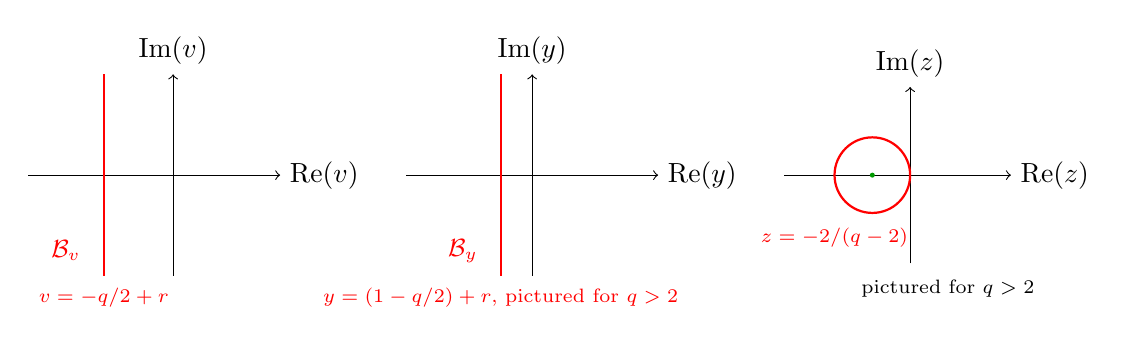
\begin{tikzpicture}[scale=0.8]
  \draw[->] (-2,0) -- (2,0) node[right] {$\mathrm{Re}(v)$}; \draw[->] (0.3,-1.6) -- (0.3,1.6) node[above] {$\mathrm{Im}(v)$};
  \draw[red,thick] (-0.8,-1.6) -- (-0.8,1.6); \node[red,font=\small] at (-1.4,-1.2) {$\mathcal B_v$};
  \node[red,font=\scriptsize] at (-0.8,-1.95) {$v = -q/2+\ii r$};
  \begin{scope}[xshift=6cm]
  \draw[->] (-2,0) -- (2,0) node[right] {$\mathrm{Re}(y)$}; \draw[->] (0,-1.6) -- (0,1.6) node[above] {$\mathrm{Im}(y)$};
  \draw[red,thick] (-0.5,-1.6) -- (-0.5,1.6); \node[red,font=\small] at (-1.1,-1.2) {$\mathcal B_y$};
  \node[red,font=\scriptsize] at (-0.5,-1.95) {$y = \left(1-q/2\right)+\ii r$, pictured for $q>2$};
  \end{scope}
  \begin{scope}[xshift=12cm]
  \draw[->] (-2,0) -- (1.6,0) node[right] {$\mathrm{Re}(z)$}; \draw[->] (0,-1.4) -- (0,1.4) node[above] {$\mathrm{Im}(z)$};
  \draw[red,thick] (-0.6,0) circle (0.6); \fill[green!60!black] (-0.6,0) circle (0.04);
  \node[red,font=\scriptsize] at (-1.2,-1.0) {$z = -2/(q-2)$};
  \node[font=\scriptsize] at (0.6,-1.8) {pictured for $q>2$};
  \end{scope}
\end{tikzpicture}
\diagramcaption{The loci $\mathcal B_v$, $\mathcal B_y$ and $\mathcal B_z$ for the $q$-state Potts model on the
circuit graph in the limit $n\to\infty$. In the $z$ plane $\mathcal B_z$ is the circle
$|z+1/(q-2)| = 1/|q-2|$, with center $z = -1/(q-2)$ and radius $1/|q-2|$.}
\end{diagram}

So we see that for the $q = 2$ Ising case, $\mathcal B_y$ is the imaginary axis in the complex $y$ plane, which maps
to itself under the inversion map $y = z^{-1}\to z$. So for the Potts model with general $q$, the locus
$\mathcal B_z$ again separates the $z$ plane into two regions. To the right, $f = \ln(q+v)$ and to the left,
$f = \ln v$; there is a non-analytic change in $f$ as one crosses the boundary $\mathcal B_v$. The image of
$\mathcal B$ in the $z$ plane is a circle that passes through $z = 0$ and
$z = \left(1-q/2\right)^{-1} = 2/(2-q) = -\left(2/(q-2)\right)$:
\begin{equation}
  \left|z+\frac{1}{q-2}\right| = \frac{1}{|q-2|}.
\end{equation}
As $q\to 2^+$, the left crossing point on $\mathcal B_z$ goes to $-\infty$, and at $q = 2$, the circle becomes the
imaginary axis. If $q<2$, then the circle crosses the positive real $z$ axis.

A general property of $\mathcal B_v$, $\mathcal B_y$, and $\mathcal B_z$ is that this locus is invariant under
complex conjugation, as a consequence of the property that (for real $q$) the coefficients of powers of $v$ in
$Z(G,q,v)$ are real. More generally, this applies for the set of discrete zeros themselves, before taking the limit
$n\to\infty$ to get the loci $\mathcal B$.

\paragraph{Zeros in the complex $q$ plane.} It is also of interest to study the zeros of $Z(G,q,v)$ in the complex
$q$ plane for fixed $v$ (say real $v$). For example for the $n\to\infty$ limit of the $G = C_n$ graph, i.e.\ the
thermodynamic limit of the 1D lattice, the locus of zeros in the $q$ plane, using
$Z(C_n,q,v) = (q+v)^n + (q-1)v^n$, is determined by the equation
\begin{equation}
  |q+v| = |v|;
\end{equation}
the solution in the $q$ plane is the circle centered at $q = -v$ with radius $|v|$, where $v = e^K-1 = e^{\beta J}-1$.

\begin{diagram}
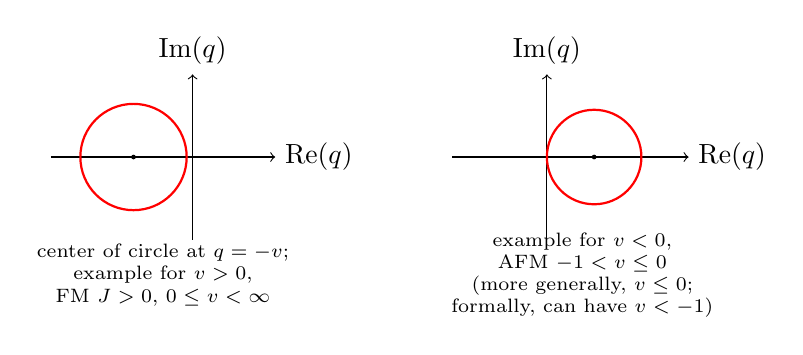
\begin{tikzpicture}[scale=0.75]
  \draw[->] (-2.4,0) -- (1.4,0) node[right] {$\mathrm{Re}(q)$}; \draw[->] (0,-1.4) -- (0,1.4) node[above] {$\mathrm{Im}(q)$};
  \draw[red,thick] (-1,0) circle (0.9); \fill (-1,0) circle (0.04);
  \node[font=\scriptsize,align=center] at (-0.5,-2.0) {center of circle at $q = -v$;\\ example for $v>0$,\\ FM $J>0$, $0\le v<\infty$};
  \begin{scope}[xshift=6cm]
  \draw[->] (-1.6,0) -- (2.4,0) node[right] {$\mathrm{Re}(q)$}; \draw[->] (0,-1.4) -- (0,1.4) node[above] {$\mathrm{Im}(q)$};
  \draw[red,thick] (0.8,0) circle (0.8); \fill (0.8,0) circle (0.04);
  \node[font=\scriptsize,align=center] at (0.6,-2.0) {example for $v<0$,\\ AFM $-1<v\le 0$\\ (more generally, $v\le 0$;\\ formally, can have $v<-1$)};
  \end{scope}
\end{tikzpicture}
\diagramcaption{The locus $\mathcal B_q$ for the circuit graph in the limit $n\to\infty$.}
\end{diagram}

Again, this locus $\mathcal B_q$ separates the complex $q$ plane into two regions, with different analytic forms for
$f$:
\begin{equation}
  f = \begin{cases}\ln(q+v) & \text{outside circle}\\ \ln v & \text{inside circle.}\end{cases}
\end{equation}

\paragraph{Chromatic zeros.} A case of particular interest is the $T = 0$ antiferromagnetic Potts model; here,
$\beta = \infty$, $J<0$, so $K = -\infty$, and $v = e^K-1 = -1$. Recall that
\begin{equation}
  Z(G,q,v=-1) = P(G,q),
\end{equation}
where $P(G,q)$ is the chromatic polynomial, counting the number of ways of assigning $q$ colors to the vertices of
the graph $G$ such that adjacent vertices have different colors. The degeneracy per vertex in the limit $n\to\infty$
is $W(\{G\},q) = \lim_{n\to\infty}[P(G,q)]^{1/n}$ and the corresponding entropy per vertex is
$S(\{G\},q) = \kB\ln[W(\{G\},q)]$, where $\{G\}$ denotes the formal limit of $G$ for $n\to\infty$. For the 1D lattice
\begin{equation}
  P(C_n,q) = (q-1)^n + (q-1)(-1)^n,
\end{equation}
and $\mathcal B_q$ is the unit circle $|q-1| = 1$. Outside this circle, $W = q-1$, where we take the principal sheet
in evaluating the $1/n$ power of $P$ for $q\in\mathbb R$, $q>2$, but only determine $|W|$ inside the circle ($P$ can
be $<0$). Inside the circle, $|W| = 1$. The maximal point where this $\mathcal B_q$ intersects the real axis is
denoted $q_c$; here, $q_c = 2$.

The discrete zeros of $P(G,q)$ in the complex $q$ plane are called chromatic zeros. In a series of papers we have
calculated these zeros for a variety of families of graphs, including strips of regular lattices with given widths
and arbitrarily great lengths, and we have determined the loci $\mathcal B_q$ in the limit of $\infty$ length. These
studies give insight into the behavior of the ground-state entropy of the Potts model on these infinite-length,
finite-width lattices. For example, the fact that for the $L_x\to\infty$ limit of the 1D lattice using $C_n$ (PBC),
$\mathcal B_q$ crosses the real axis at the maximal point $q_c = 2$, can be seen as the manifestation in the $q$
plane of the $T = 0$ singularity of the Ising AFM, embodied in the behavior of $\mathcal B_y$, which crosses the real
$y = e^K$ axis at $y = 0$.

In effect, one can think of the locus as a subvariety in a $\mathbb C^2$ space spanned by $(q,y)$, such that
$\mathcal B_q$ is the slice for a given $y$ such as $y = 0$, and $\mathcal B_y$ is the slice for a given $q$ such as
$q = 2$.
